\documentclass[conference]{IEEEtran}
\IEEEoverridecommandlockouts
\usepackage{cite}
\usepackage{amsmath,amssymb}
\usepackage{graphicx}
\usepackage{booktabs}
\usepackage{tabularx}
\usepackage{array}
\usepackage{multirow}
\usepackage{url}
\usepackage{balance}
\usepackage{stfloats}
\usepackage[hidelinks,pdfusetitle]{hyperref}
\graphicspath{{figures/}}
\urlstyle{same}
\hypersetup{pdftitle={Investigating Weisfeiler–Lehman Graph Kernels for Fine-Grained Plant Stress Classification Using Phenotypic Features},pdfauthor={Yerneni Vishnu Vardhan; Muppagowni Vamsidhar; Bala Bharath Chandra Sai; Merugumala Sandeep; Chilukuri Subrahmanya Sri Prakash; S Sriram},pdfsubject={IEEE-style professor-review manuscript},pdfkeywords={plant stress phenotyping, graph kernels, Weisfeiler-Lehman, OLID-I, feature graph construction}}
\newcommand{\AccessibleGraphic}[2]{#2}
\newcommand{\meanSD}[2]{#1\,\ensuremath{\pm}\,#2}
\newcommand{\pp}{\,\text{percentage points}}
\title{Investigating Weisfeiler–Lehman Graph Kernels for Fine-Grained Plant Stress Classification Using Phenotypic Features}
% \author{
% \IEEEauthorblockN{Yerneni Vishnu Vardhan\\Muppagowni Vamsidhar\\Bala Bharath Chandra Sai}
% \IEEEauthorblockA{\textit{Department of Computer Science and Engineering}\\\\[0.3ex]\textit{Amrita Vishwa Vidyapeetham, India}}
% \and
% \IEEEauthorblockN{Merugumala Sandeep\\Chilukuri Subrahmanya Sri Prakash\\S Sriram}
% \IEEEauthorblockA{\textit{Department of Computer Science and Engineering}\\\\[0.3ex]\textit{Amrita Vishwa Vidyapeetham, India}}
% }

\begin{document}
\maketitle
\begin{abstract}
Plant stress phenotyping increasingly uses image analysis, but conventional classifiers usually treat image-derived descriptors as independent coordinates and do not explicitly represent relationships between traits. We evaluated whether representing leaf descriptors as labelled graphs improves discrimination among crop--condition categories in the Open Leaf Image Dataset I (OLID-I). The supplied pipeline describes an excess-green and Otsu-thresholding segmentation stage followed by extraction of 38 shape, color, texture, and regional descriptors. Of 4,749 records in the stored feature table, 4,387 passed the pipeline's mask-quality filter and 362 (7.6\%) were excluded. Each retained record was represented as a 38-node graph with feature identity and training-fold quantile bin encoded in each node label. Five topologies---correlation, feature-similarity $k$-nearest neighbors, feature-family, spatial/regional, and hybrid---were compared using normalized Weisfeiler--Lehman subtree kernels at heights 0--3 and a class-balanced support vector machine. Four flat-feature classifiers were evaluated on the same stratified five-fold splits. The best graph-kernel configuration was the hybrid topology at height 2, with accuracy of 44.31\% $\pm$ 0.72\% and macro-F1 of 42.79\% $\pm$ 0.95\% (mean $\pm$ standard deviation across folds). The Random Forest baseline achieved 58.54\% $\pm$ 1.47\% accuracy and 54.99\% $\pm$ 1.35\% macro-F1, outperforming all evaluated graph-kernel configurations. The quality audit also revealed non-uniform retention: acceptance ranged from 72.68\% for tomato records to 99.90\% for ash gourd, and was 51.69\% for the LM condition. These results show that graph construction and WL height affect performance, but the evaluated graph representations did not improve full 57-class prediction over flat handcrafted-feature baselines. The results also identify segmentation-driven selection bias as a material limitation for plant stress phenotyping on this feature table.
\end{abstract}

\begin{IEEEkeywords}
plant stress phenotyping, OLID-I, graph kernels, Weisfeiler--Lehman, handcrafted features, segmentation quality
\end{IEEEkeywords}

\section{Introduction}

Plant stress phenotyping supports the assessment of disease, pest injury, and nutrient deficiencies that influence crop growth and productivity. Image-based methods can provide non-destructive measurements at a scale that is difficult to achieve through manual inspection, and machine-learning systems are increasingly used to classify visible symptoms from plant images \cite{Mohanty2016,Gill2022,Pacal2024}. The reliability of an automated phenotyping system, however, depends on more than the choice of classifier. Image quality, segmentation, class imbalance, and the relation between extracted traits and target labels can all affect a model's measured performance.

The Open Leaf Image Dataset I (OLID-I) was released to support plant-stress recognition across eight crop species and 57 categories that include healthy leaves, nutrient deficiencies, pest damage, diseases, and combined conditions \cite{Orka2023}. Its diversity makes the dataset useful for asking whether a representation can distinguish visually related crop--condition classes, rather than only separating healthy leaves from a single disease. Recent work has explored both deep architectures for OLID-I and graph-based representations of image-derived plant traits \cite{Karthikeyan2026,Sriram2026}. These studies motivate further investigation of how trait relationships should be encoded and when relational representations offer practical benefit.

Handcrafted image descriptors summarise leaf geometry, color, texture, and regional differences. In a conventional feature vector, a classifier receives the descriptor values but does not explicitly model a network of relations among descriptors. A graph representation offers a way to define each descriptor as a node and connect nodes according to a specified relation, such as statistical association, similarity across images, membership in a feature family, or regional structure. A Weisfeiler--Lehman (WL) subtree kernel then compares graphs by repeatedly combining each node's current label with the labels of its neighbours and counting the resulting patterns \cite{Shervashidze2011}. The usefulness of this approach depends on both the graph topology and the depth of label refinement: a graph that is too sparse may miss informative interactions, while a dense graph or excessive refinement can generate a large and less discriminative representation.

Graph-based plant phenotyping is not a new idea. For example, Sriram and Ramraj introduced a perceptual graph-kernel framework~\cite{Sriram2026} for image-derived trait interactions, while graph-convolutional architectures have also been investigated for leaf-disease recognition. The present study takes a narrower, comparative approach: rather than introducing a new kernel, it evaluates five alternative ways to connect the same 38 handcrafted descriptors and tests how WL height changes their classification performance on the 57-class OLID-I task. Flat-feature baselines are evaluated on the same folds to test whether the graph representation improves predictive performance in this setting.

A second concern arises before classification. The supplied segmentation pipeline accepts or excludes records according to the proportion of an image selected as leaf mask. If the acceptance mechanism differs by crop or condition, classification results measured only on retained records may not represent the original dataset population. We therefore analyse crop- and condition-specific acceptance alongside the graph-kernel experiments.

The study addresses three questions: (1) how does graph topology affect the performance of a WL subtree-kernel classifier on the full crop--condition task? (2) does a graph-kernel representation outperform standard classifiers using the same descriptors? and (3) is the mask-quality filter associated with materially different data-retention rates across crops and conditions? The contribution is a controlled benchmark and a data-quality audit, not a claim that graph kernels provide state-of-the-art plant stress recognition.


\begin{figure*}[!t]
\centering
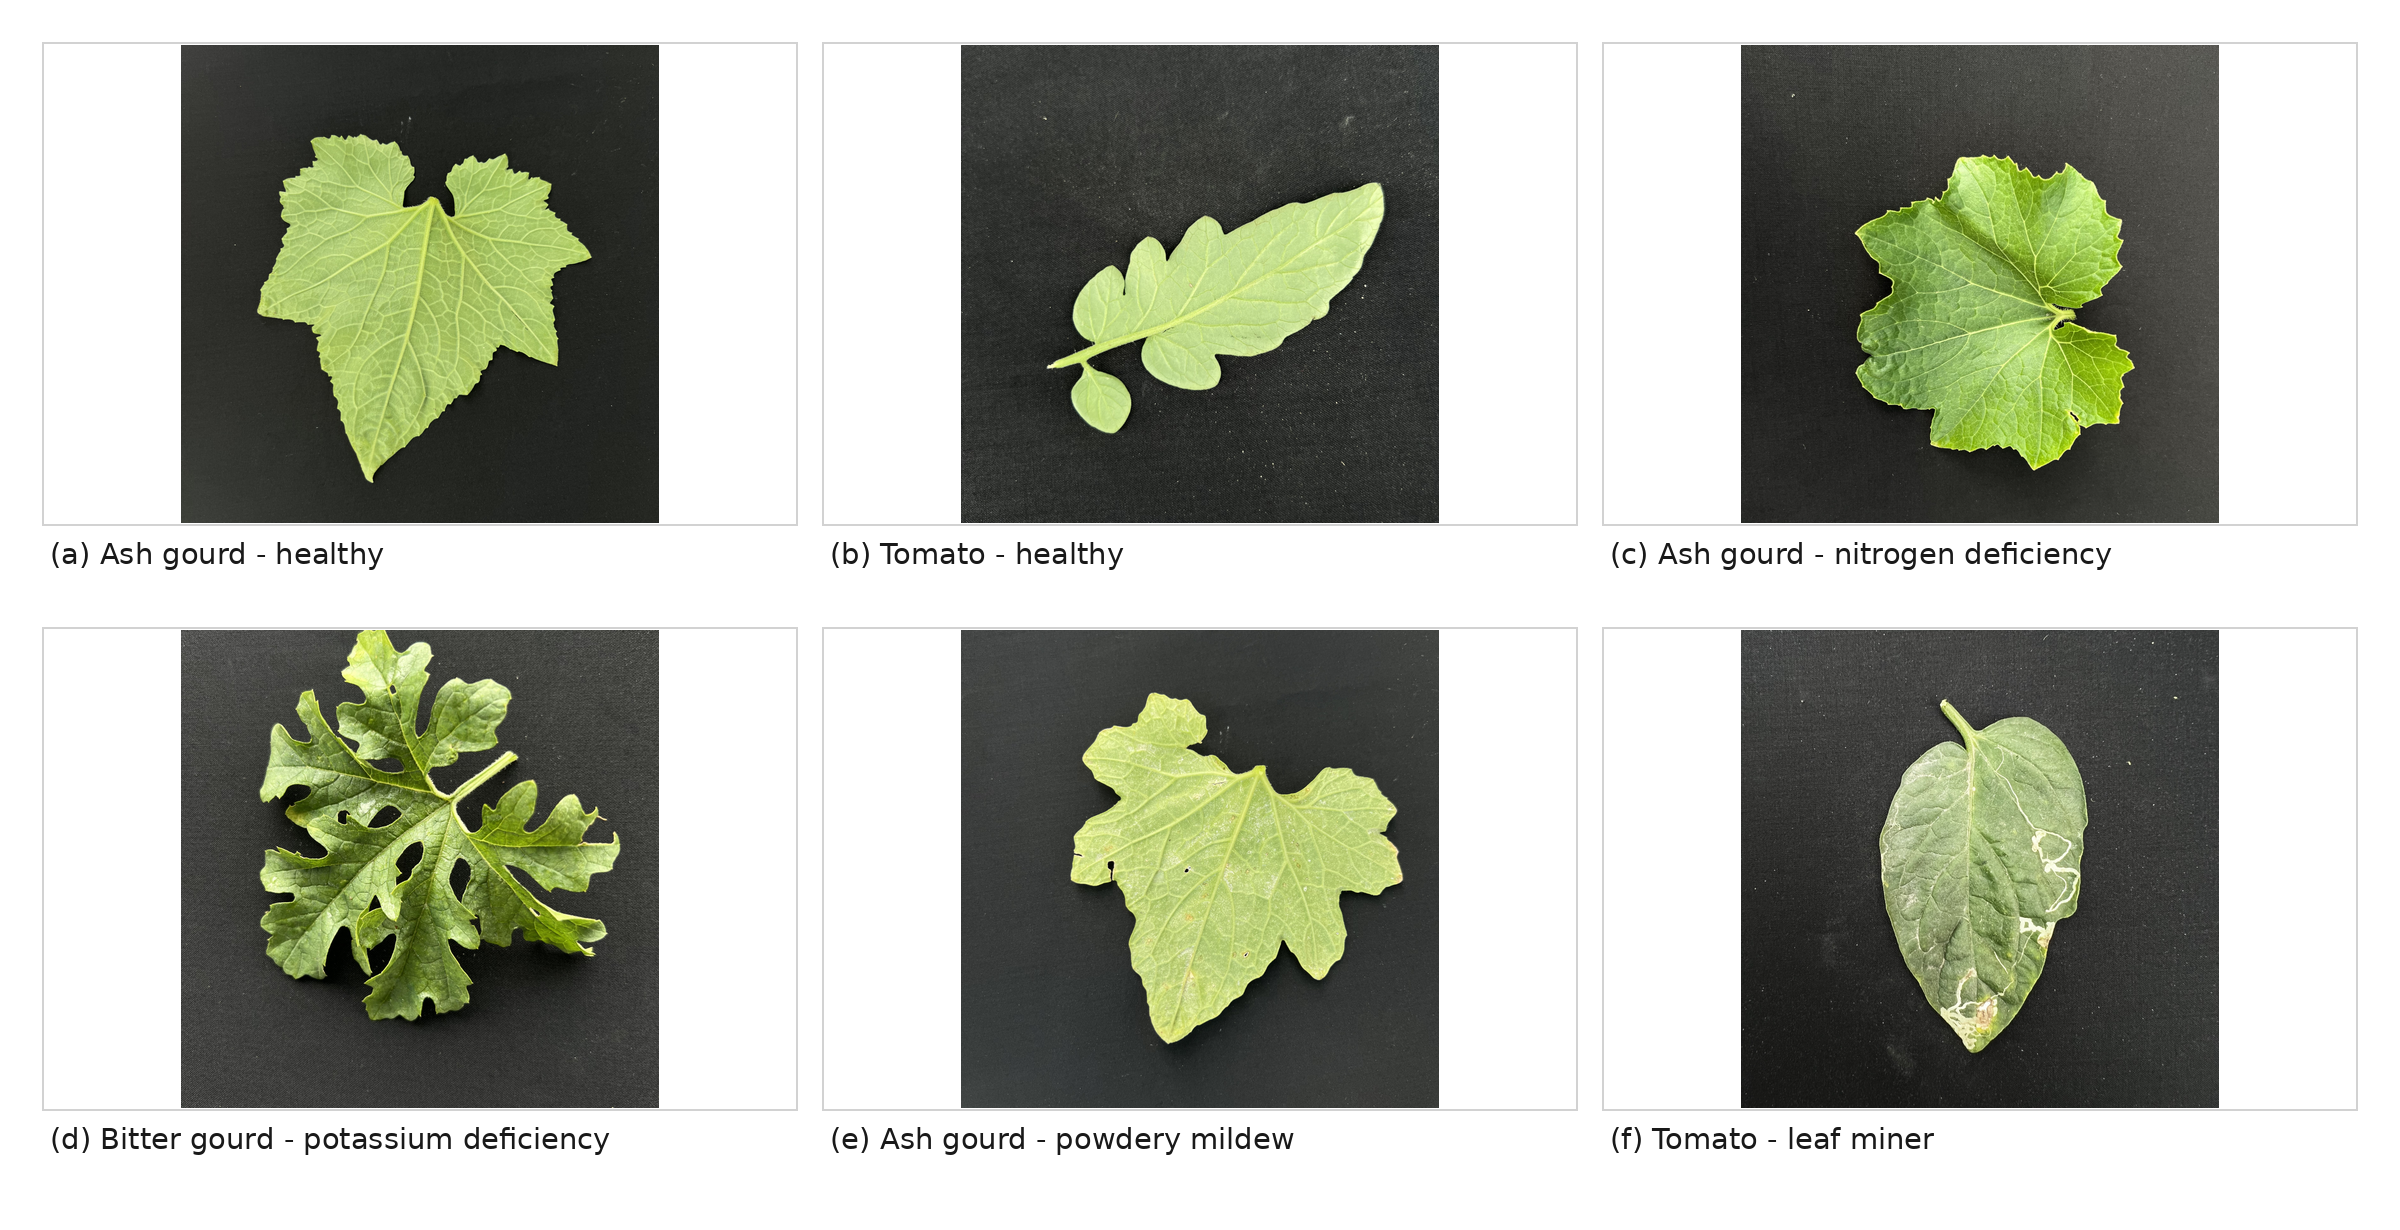
\includegraphics[width=0.96\textwidth]{figures/fig1_representative_leaf_images.png}
\caption{Representative OLID-I leaf images supplied for visual illustration, showing healthy leaves, nutrient-deficiency symptoms, and biotic stress. This montage is illustrative and does not define a separate evaluation subset. The acceptance audit uses all 4,749 feature-table records, while classifier metrics use the 4,387 records that passed the stored filter. Dataset source: OLID-I~\cite{Orka2023}.}
\label{fig:examples}
\end{figure*}

\section{Materials and methods}

\begin{figure*}[!t]
    \centering
    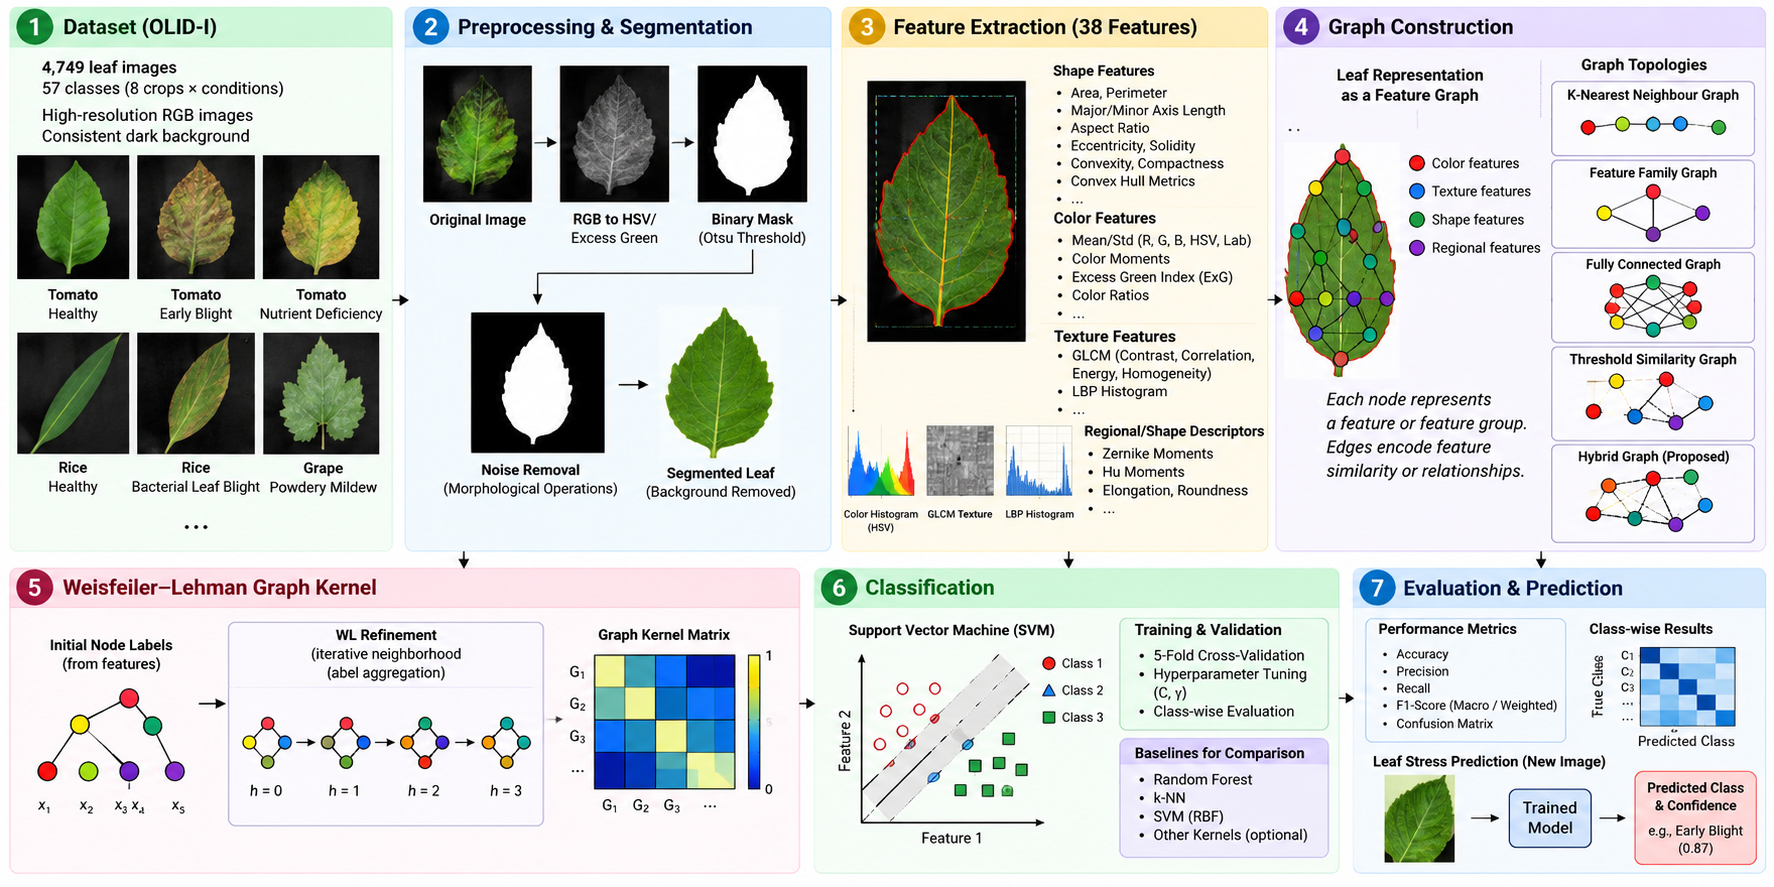
\includegraphics[width=\textwidth]
    {Plant Leaf Stress Classification Workflow-1.png}
    \caption{Overview of the proposed workflow for evaluating
    graph construction strategies and Weisfeiler--Lehman graph
    kernels for plant-stress classification using OLID-I.}
    \label{fig:study_workflow}
\end{figure*}


\subsection{Dataset and prediction task}

The experiments used the supplied project table, \texttt{olid\_full\_features.csv}, which contains 4,749 records linked to the OLID-I image collection described by Orka et al.~\cite{Orka2023}. The source collection covers ash gourd, bitter gourd, bottle gourd, cucumber, eggplant, ridge gourd, snake gourd, and tomato. Each observation is assigned a \texttt{class} value formed from its crop and condition label; combined conditions are represented as their own target categories. The evaluated task is therefore a 57-class crop--condition classification problem, not a binary healthy-versus-stressed task and not a multi-output prediction of separate labels.

The current re-analysis starts from the stored feature table rather than re-running image segmentation on the original image files. The feature-extraction and quality-control procedures below describe the accompanying project source code. Consequently, classification metrics reported here are conditional on the features and quality flags already stored in that table. The original image collection remains the source dataset and should be retrieved from its public repository for a fully end-to-end rerun.

A small image subset was supplied for visual illustration only. Fig.~\ref{fig:examples} shows six representative leaves spanning healthy, nutritional-deficiency, and biotic-stress conditions. These examples are not a separate modeling cohort and do not redefine the classification task. The analysis begins from all 4,749 rows in the full derived-feature table. Classifier metrics are computed on the 4,387 records that passed the stored quality filter, while the acceptance audit compares accepted and excluded records across the full table. The full high-resolution image archive is larger than the illustration subset and is not repackaged with this manuscript.

\subsection{Segmentation, quality control, and handcrafted descriptors}

The supplied image-processing code converts each image to RGB and calculates an excess-green response after normalizing each channel by the pixel-wise sum of red, green, and blue intensities:
\begin{equation}
\mathrm{ExG}=2\frac{G}{R+G+B}-\frac{R}{R+G+B}-\frac{B}{R+G+B},
\label{eq:exg}
\end{equation}
where zero channel sums are protected against division by zero. The response is min--max normalized to an 8-bit image, thresholded using Otsu's method \cite{Otsu1979}, and refined by morphological opening and closing with a $5\times5$ elliptical structuring element for two iterations each. The largest external contour is retained as the leaf mask. The pipeline labels a mask as failed when its area ratio is below 0.01 (including an empty mask) and as suspicious when its ratio exceeds 0.98; records with a mask ratio between 0.01 and 0.98 are marked as accepted.

Thirty-eight numerical descriptors were computed. Ten describe shape and geometry (area, perimeter, aspect ratio, circularity, extent, solidity, convex-hull area, major and minor axis lengths, and eccentricity); six summarise RGB channels; six summarise HSV channels; six summarise CIELAB channels; two are derived color ratios; four are gray-level co-occurrence matrix (GLCM) texture statistics; and four describe regional color differences between a central region and the surrounding edge region. The GLCM feature implementation follows the general gray-level co-occurrence framework \cite{Haralick1973} and operates on the grayscale crop defined by the leaf bounding box, rather than applying the binary mask to every pixel in that crop. Background pixels within this crop may therefore affect the texture descriptors. The feature names, families, and operational definitions are provided in the supplementary feature dictionary. A dataset-specific caveat is important: the OLID-I release describes a consistent black background and states that segmentation is not required for the dataset as released~\cite{Orka2023}. Accordingly, the excess-green/Otsu stage analysed here is an additional project-pipeline choice, not a requirement of the benchmark. The resulting mask rejection rates should therefore be interpreted as an audit of this implementation and not as evidence that the original dataset images are intrinsically unusable.



\subsection{Quality-filter selection audit}

We retained records whose stored \texttt{quality\_flag} equalled \texttt{ACCEPT}. We compared the original, accepted, and excluded counts by crop and by condition using the saved project audit tables. Acceptance rate was calculated as accepted records divided by original records within each group. This analysis is descriptive: it establishes differential retention but does not infer the cause of each failed mask or quantify the stress-classification performance of rejected images.

\subsection{Feature-graph construction}

Each accepted sample was encoded as a graph with 38 nodes, one per descriptor. The same set of feature nodes was used across graph types. Continuous descriptor values were discretized into three quantile bins (low, medium, and high). The bin boundaries were fit to the training portion of each cross-validation split only, and the initial node label retained feature identity (for example, \texttt{mean\_H::Low} is distinct from \texttt{area::Low}). Each topology was also fitted using training-fold feature data only. Five graph constructors were compared:

\begin{enumerate}
\item \textbf{Correlation graph:} an undirected edge connects feature pairs whose absolute Pearson correlation in the training fold is at least 0.70.
\item \textbf{Feature-similarity k-nearest-neighbour graph:} features are standardized across training samples and represented as vectors over those samples. Each feature is connected to its three nearest other feature vectors under Euclidean distance; the resulting relation is treated as an undirected graph.
\item \textbf{Feature-family graph:} features within each pre-defined family form a clique. Between each pair of families, one bridge edge connects the feature pair with the largest absolute training-fold correlation.
\item \textbf{Spatial/regional graph:} the four regional descriptors are connected within core and edge groups and by matching core--edge pairs; global descriptors are linked to regional descriptors when their absolute training-fold correlation is at least 0.60.
\item \textbf{Hybrid graph:} the union of a correlation graph with threshold 0.80, the feature-family graph, and a spatial/regional graph with threshold 0.70. The hybrid topology does not include the k-nearest-neighbour edges.
\end{enumerate}

The resulting graphs are deterministic given the input data and split. Figure~\ref{fig:topologies} visualises the topologies obtained in the first training fold; model evaluation reconstructs them separately within each fold. The average numbers of edges observed during five-fold evaluation are reported in Table~\ref{tab:topology}.

\begin{table}[!htbp]
\centering
\caption{Feature-graph definitions and mean edge counts across the five training folds.}
\label{tab:topology}
\small
\begin{tabularx}{\columnwidth}{>{\raggedright\arraybackslash}p{0.23\columnwidth}>{\raggedright\arraybackslash}Xr}
\toprule
Topology & Construction rule & Mean edges \\
\midrule
Correlation & Undirected edge when absolute Pearson correlation $|r|\geq0.70$ on the training fold. & 71.8 \\
Feature-similarity kNN & Each feature is a vector across training samples; connect its $k=3$ nearest feature vectors and symmetrize. & 81 \\
Feature-family & Cliques within seven descriptor families plus one maximum-absolute-correlation bridge for every pair of families. & 124 \\
Spatial/regional & Core and edge regional cliques, matching core--edge links, and global-to-regional links above $|r|\geq0.60$. & 19 \\
Hybrid & Union of correlation threshold 0.80, feature-family edges, and spatial/regional links (threshold 0.70); excludes kNN edges. & 147 \\
\bottomrule
\end{tabularx}
\smallskip
\begin{minipage}{0.96\linewidth}\footnotesize The same 38 feature nodes were used for every topology. Correlation and feature-similarity structures were reconstructed independently within each training fold; edge counts are averaged across folds.\end{minipage}
\end{table}

\begin{figure*}[!t]
\centering
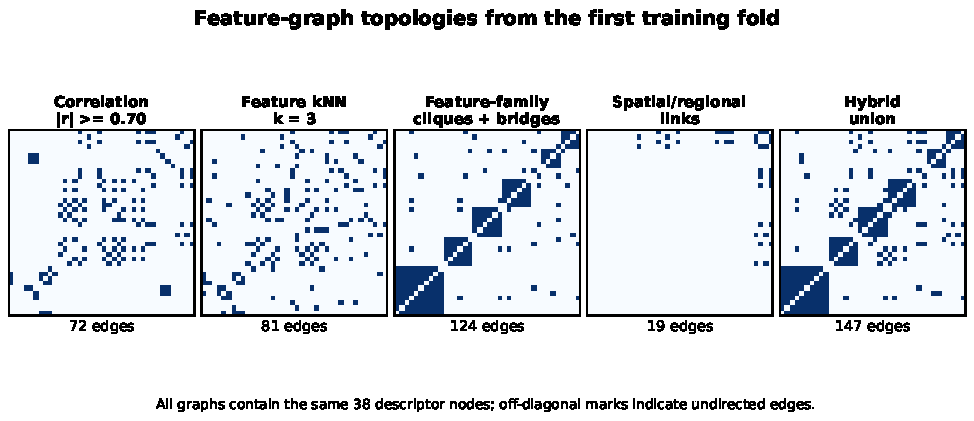
\includegraphics[width=0.97\textwidth]{figures/fig5_graph_topologies.pdf}
\caption{Illustrative adjacency matrices for the five graph constructors, fitted to the first training fold. The plots show connectivity only; the graph structures were reconstructed separately for every fold used in evaluation.}
\label{fig:topologies}
\end{figure*}

\subsection{Weisfeiler--Lehman subtree kernel}

For a labelled graph $G=(V,E)$, each node $v$ begins with its feature-specific discretized label $l_0(v)$. At WL iteration $t$, the current label is combined with the sorted multiset of neighbouring labels to form a signature,
\begin{equation}
l_{t+1}(v)=\operatorname{compress}\!\left(l_t(v),\operatorname{sort}\{l_t(u):u\in N(v)\}\right),
\label{eq:wl}
\end{equation}
where the compression map is learned from training graphs only. For each graph and each maximum height $H\in\{0,1,2,3\}$, the feature map $\Phi_H(G)$ contains counts of labels from all iterations $0,\ldots,H$; it is not restricted to the labels from the final iteration alone. Unseen validation signatures are treated as out-of-vocabulary labels and do not add dimensions to the training vocabulary.

The graph similarity kernel is the cosine-normalized dot product of the accumulated WL label-count vectors:
\begin{equation}
K_H(G_i,G_j)=\frac{\langle\Phi_H(G_i),\Phi_H(G_j)\rangle}{\|\Phi_H(G_i)\|_2\,\|\Phi_H(G_j)\|_2}.
\label{eq:kernel}
\end{equation}
A support vector machine (SVM) using the precomputed kernel, penalty parameter $C=1$, and balanced class weights performs the 57-class prediction \cite{Cortes1995}. We evaluated every combination of five graph types and four WL heights across the same five folds.

\subsection{Flat-feature baselines and cross-validation}

Four standard classifiers were trained on the same 38-dimensional descriptors: an SVM with a radial basis function kernel ($C=1$), a linear SVM ($C=1$), a Random Forest with 300 trees, and a $k$-nearest-neighbour classifier ($k=5$). The SVM models used balanced class weights; the Random Forest used balanced-sub-sample class weights. A standard scaler was fitted only on the training fold and then applied to the validation fold. The Random Forest implementation followed the project's fixed configuration and used random seed 42 \cite{Breiman2001}. No hyperparameter search was performed in this study; these are fixed-configuration comparisons, not a tuned leaderboard. For the topology-specific summary, the height with the highest mean macro-F1 was selected from the same five folds used to report its score. The selected-height summaries are therefore subject to model-selection optimism and are descriptive, not unbiased final estimates of a selected model.

All classifiers used stratified five-fold cross-validation with shuffling and random seed 42. The same fold assignment was used for all graph-kernel and flat-feature models. Graph edges, feature discretization, scaling, WL label mappings, and WL feature vocabularies were determined without using labels or feature statistics from the corresponding validation fold. This design reduces information leakage from preprocessing and topology construction. It does not constitute an independent external test: each image appears in a validation fold once within this single five-fold partition.

We report accuracy, macro-F1, weighted-F1, macro precision, macro recall, and balanced accuracy. Macro-F1 is the unweighted average of class-specific F1 scores and therefore gives equal weight to each class irrespective of class prevalence. Weighted-F1 weights class-specific F1 scores by the number of true observations in each class. Results are presented as the mean and sample standard deviation across the five folds. The standard deviations describe fold-to-fold variation and are not confidence intervals.

\subsection{Implementation and data provenance}

The project uses Python, NumPy, pandas, scikit-learn, NetworkX, and SciPy sparse matrices for feature processing, graph construction, kernel assembly, and classification; scikit-learn provides the classification and preprocessing implementations \cite{Pedregosa2011}. The re-analysis package includes the fold-level metric files, aggregation scripts, fold assignments, feature dictionary, and figure-generation script. The cached classification outputs in the supplied notebooks were not used for the reported WL results because they were inconsistent with the source-level feature-identity labels and accumulated subtree representation. The WL scores in this manuscript were recomputed from the saved feature table using the documented fold-safe logic.



\section{Results}

\subsection{Descriptor distributions and inter-feature dependence}
The full-table descriptor distributions are heterogeneous. As illustrated in Fig.~\ref{fig:featuredist}, some geometric and texture variables are strongly right-skewed, while several color-channel summaries occupy narrower ranges. These shape differences support the use of fold-fitted scaling for distance-based baselines and training-fold quantile bins for the graph-node labels. The distributions themselves do not imply that any feature is diagnostic of a particular stress condition; they are included to describe the numerical input representation and its scale characteristics.

The correlation matrix in Fig.~\ref{fig:featurecorr} shows clusters of related descriptors, including relationships among geometry, color summaries, and regional measurements. Such redundancy makes graph construction consequential: a correlation-based graph may connect redundant measures, while feature-family construction encodes an a priori organization. The matrix is a descriptive visualization of the stored feature table; the actual graph edges used for evaluation were reconstructed from each training fold to avoid using validation-fold feature statistics.


\begin{figure*}[!t]
\centering
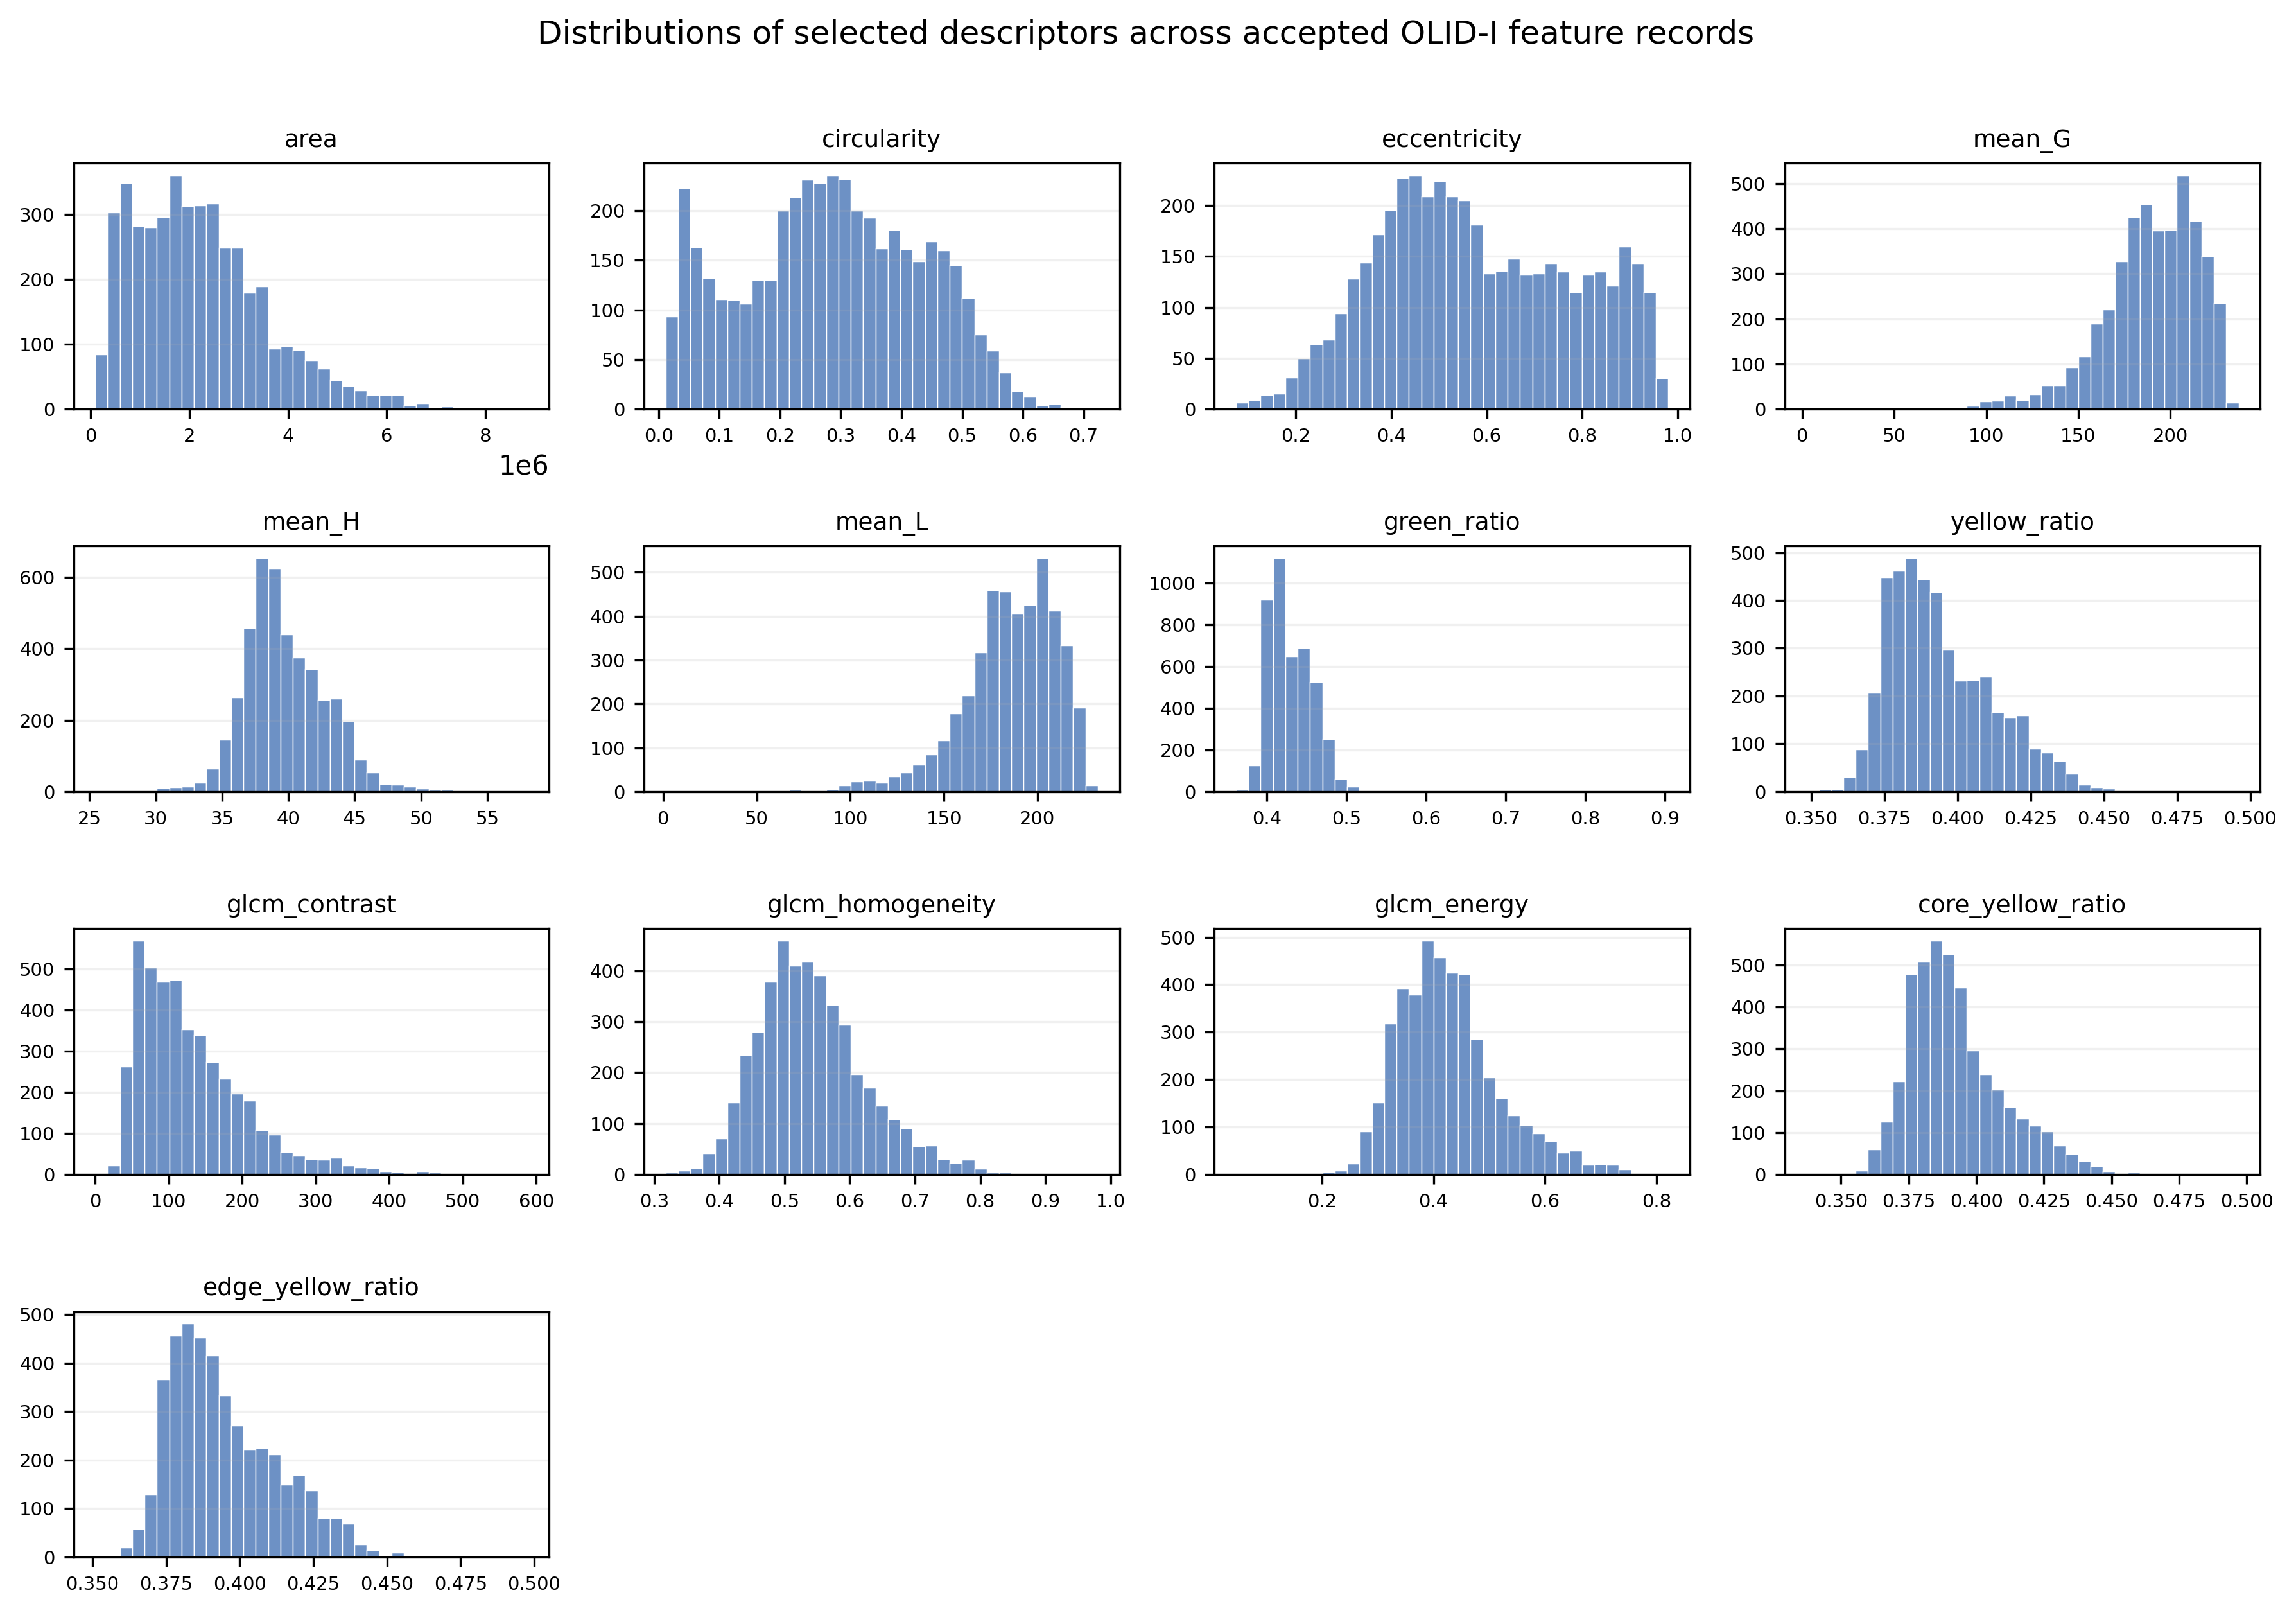
\includegraphics[width=0.97\textwidth]{figures/fig3_feature_distributions.png}
\caption{Distributions of selected shape, color, texture, and regional descriptors in the saved full-dataset feature table. The plots are descriptive and illustrate skew, concentration, and scale differences; they are not evidence of separability between classes by themselves.}
\label{fig:featuredist}
\end{figure*}

\begin{figure}[!t]
\centering
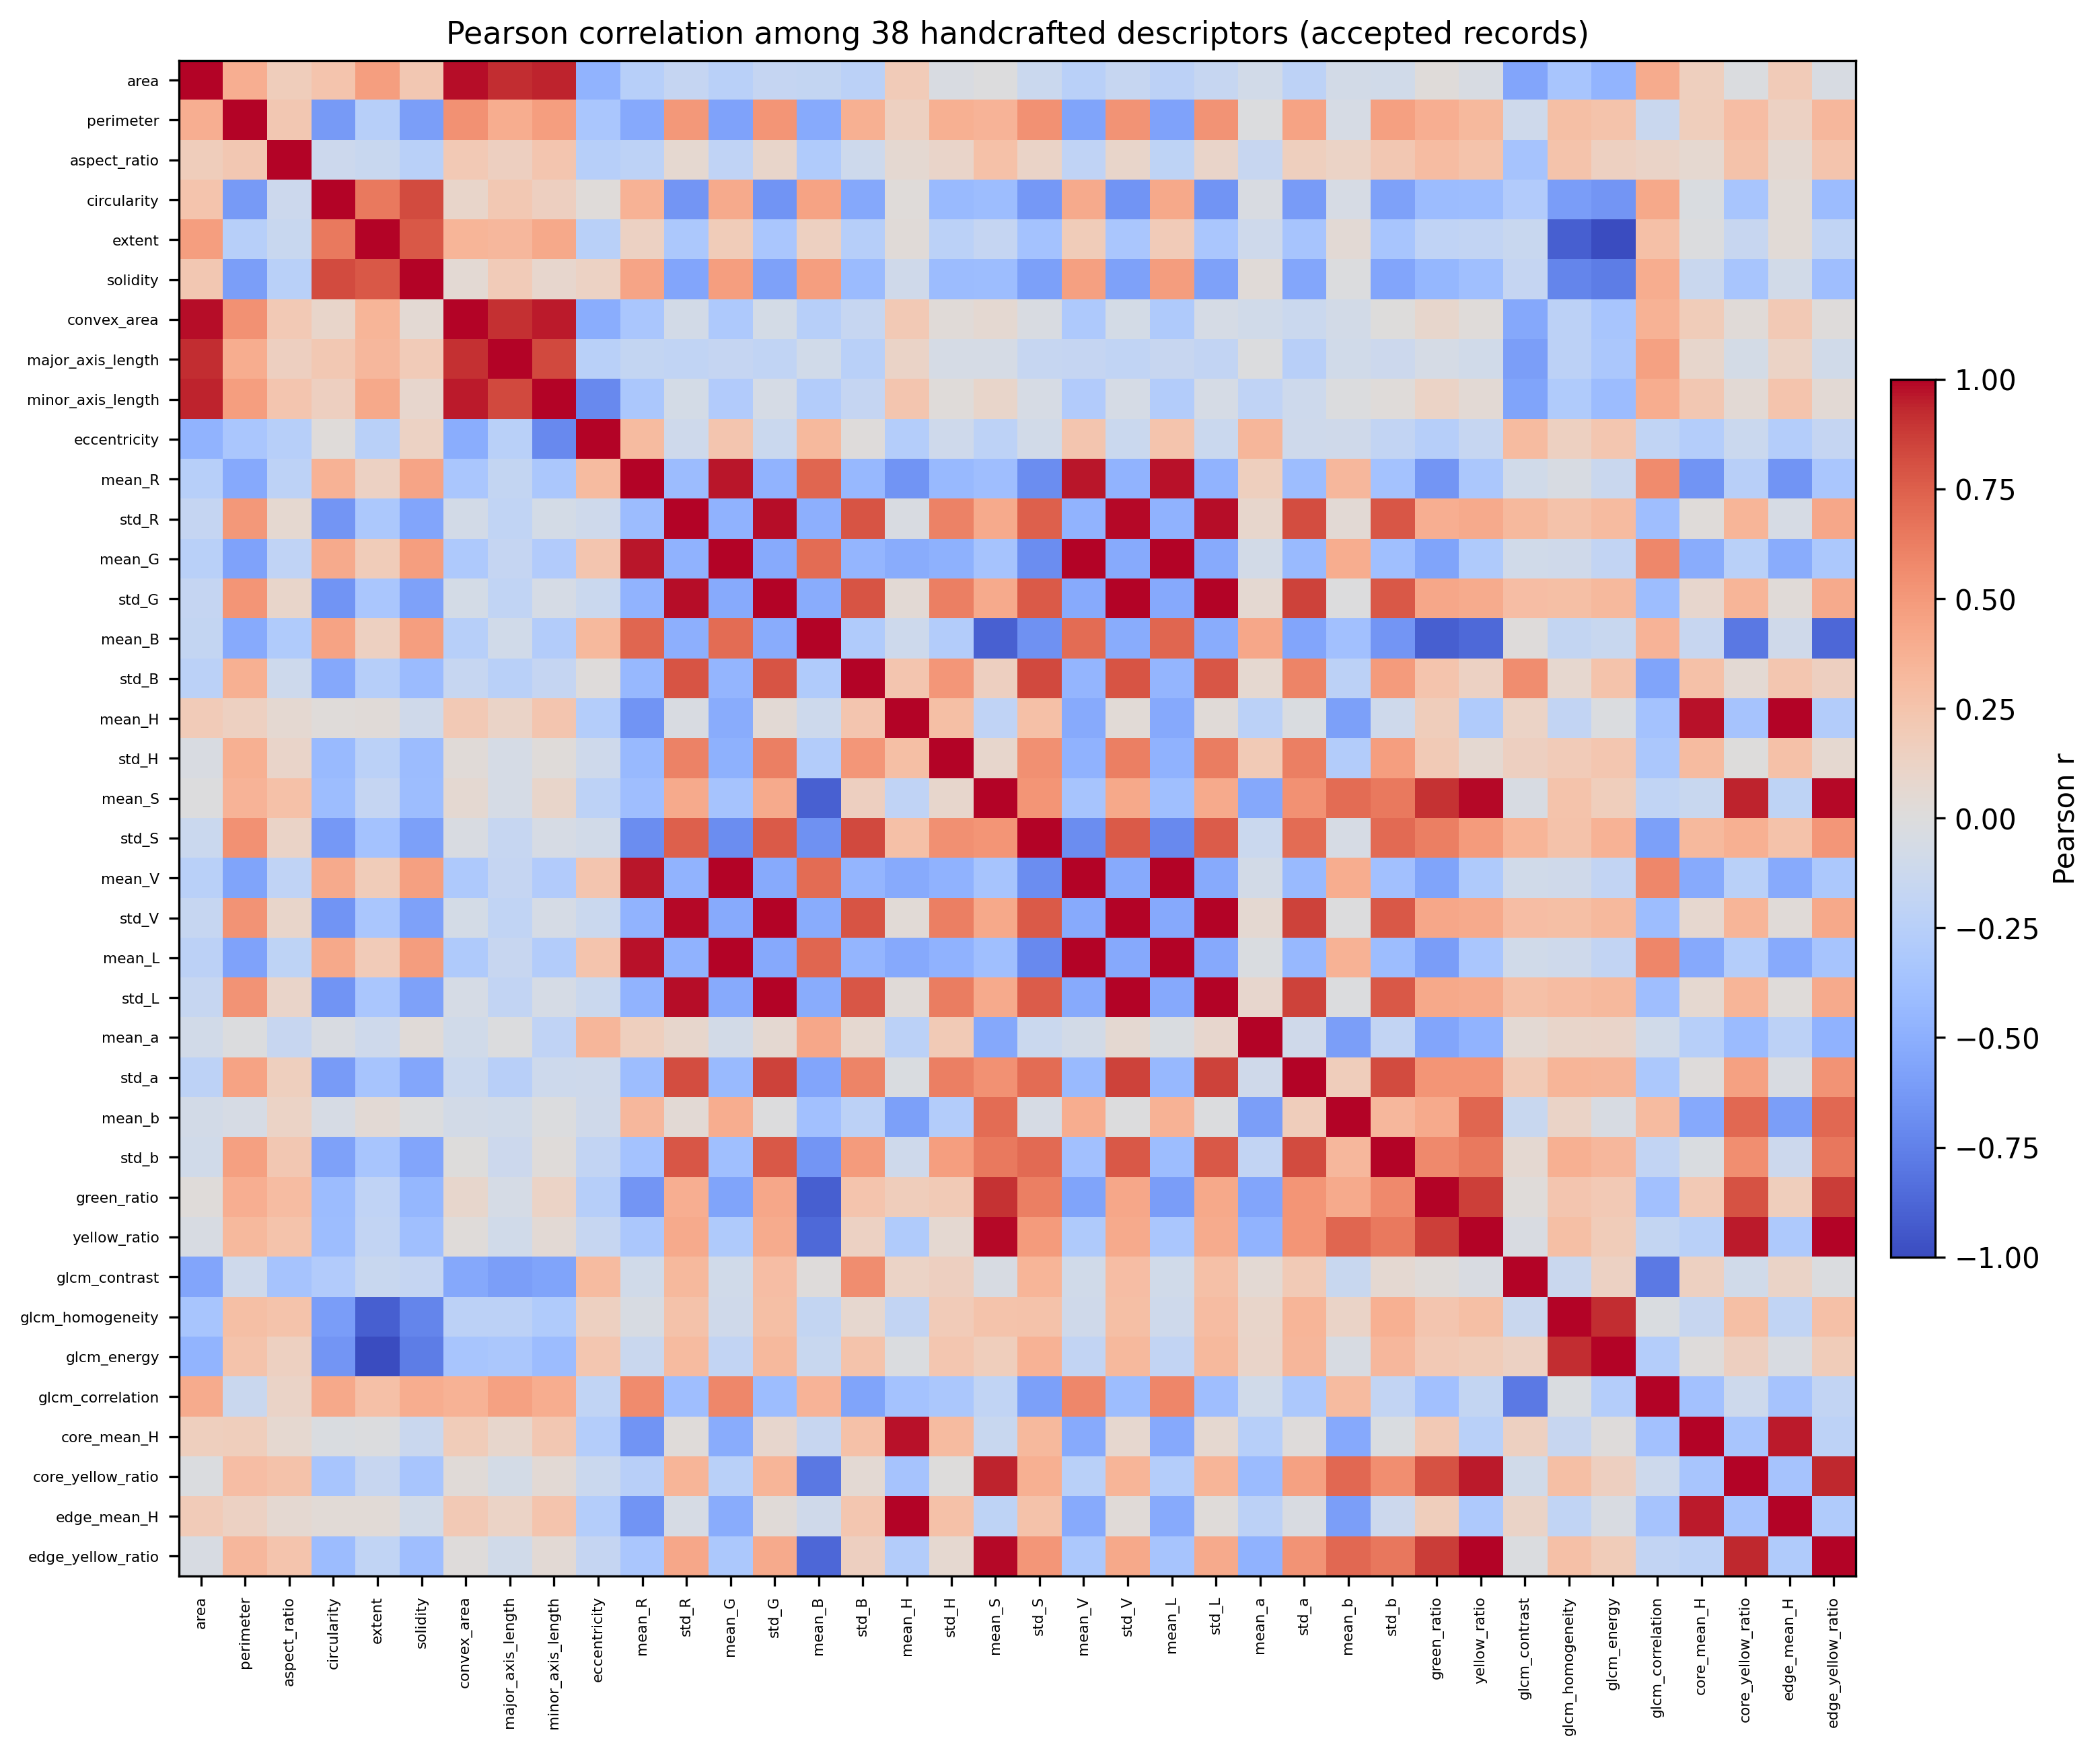
\includegraphics[width=\columnwidth]{figures/fig4_feature_correlation_heatmap.png}
\caption{Pearson correlation matrix for the 38 handcrafted descriptors. Strongly related groups motivate the comparison of correlation-aware and feature-family graph constructions.}
\label{fig:featurecorr}
\end{figure}

\subsection{Data retention and selection bias}

Of 4,749 rows in the source feature table, 4,387 were accepted and 362 excluded, corresponding to a 7.62\% overall exclusion rate. The project audit attributed 349 exclusions to empty or very small masks and 13 to masks covering more than 98\% of the image. Retention varied materially across crops (Table~\ref{tab:dataset}; Figure~\ref{fig:acceptance}). Tomato had the lowest crop-level acceptance rate (72.68\%), with 218 of 798 records excluded. Ridge gourd acceptance was 88.25\%; by contrast, ash gourd acceptance was 99.90\%, with only one of 997 records excluded.

Acceptance also differed by condition. The LM condition had 107 accepted out of 207 records (51.69\% acceptance; 100 excluded). Other lower-retention condition categories included PLEI (73.75\%) and PLEI\_MIT (80.00\%). These differences show that the mask filter is not missing at random with respect to the dataset's recorded crop and condition labels. The current classification evaluation, which uses only accepted records, consequently estimates performance on a selected subset rather than on all 4,749 source records. The audit does not establish whether exclusions are caused by symptom morphology, acquisition conditions, background similarity, or some combination of factors.

\begin{table*}[!t]
\centering
\caption{Record retention after the stored segmentation-quality filter.}
\label{tab:dataset}
\small
\begin{tabular}{lrrrr}
\toprule
Group & Original & Accepted & Excluded & Acceptance (\%) \\
\midrule
All records & 4,749 & 4,387 & 362 & 92.38 \\
tomato & 798 & 580 & 218 & 72.68 \\
ridge gourd & 434 & 383 & 51 & 88.25 \\
bitter gourd & 785 & 742 & 43 & 94.52 \\
bottle gourd & 345 & 332 & 13 & 96.23 \\
cucumber & 249 & 240 & 9 & 96.39 \\
eggplant & 685 & 662 & 23 & 96.64 \\
snake gourd & 456 & 452 & 4 & 99.12 \\
ash gourd & 997 & 996 & 1 & 99.90 \\
\bottomrule
\end{tabular}
\smallskip
\begin{minipage}{0.94\linewidth}\footnotesize The full table contains 4,749 records, of which 4,387 were accepted (92.38\%) and 362 were excluded (7.62\%). The source audit attributes 349 exclusions to empty or tiny masks and 13 to masks occupying more than 98\% of the image.\end{minipage}
\end{table*}

\begin{figure*}[!t]
\centering
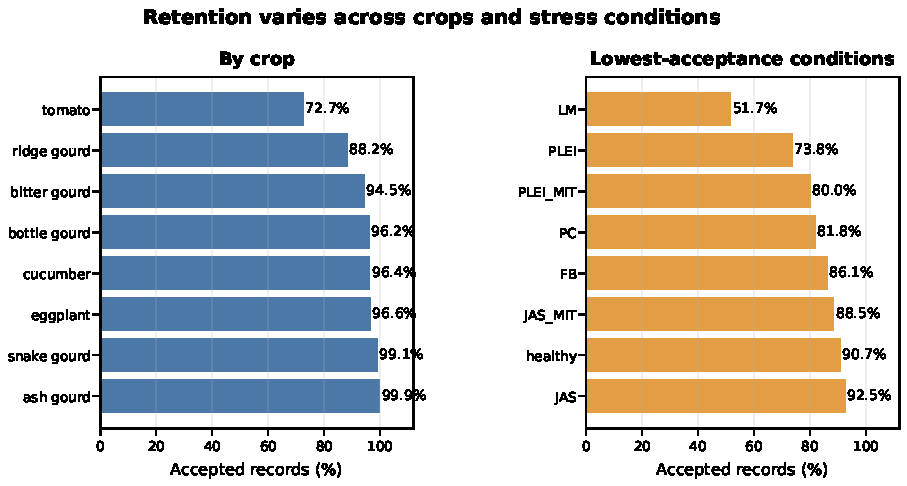
\includegraphics[width=0.97\textwidth]{figures/fig6_acceptance_audit.pdf}
\caption{Selection audit for the mask-quality filter. The right panel shows the eight conditions with the lowest acceptance rates in the project audit.}
\label{fig:acceptance}
\end{figure*}

\begin{figure}[!t]
\centering
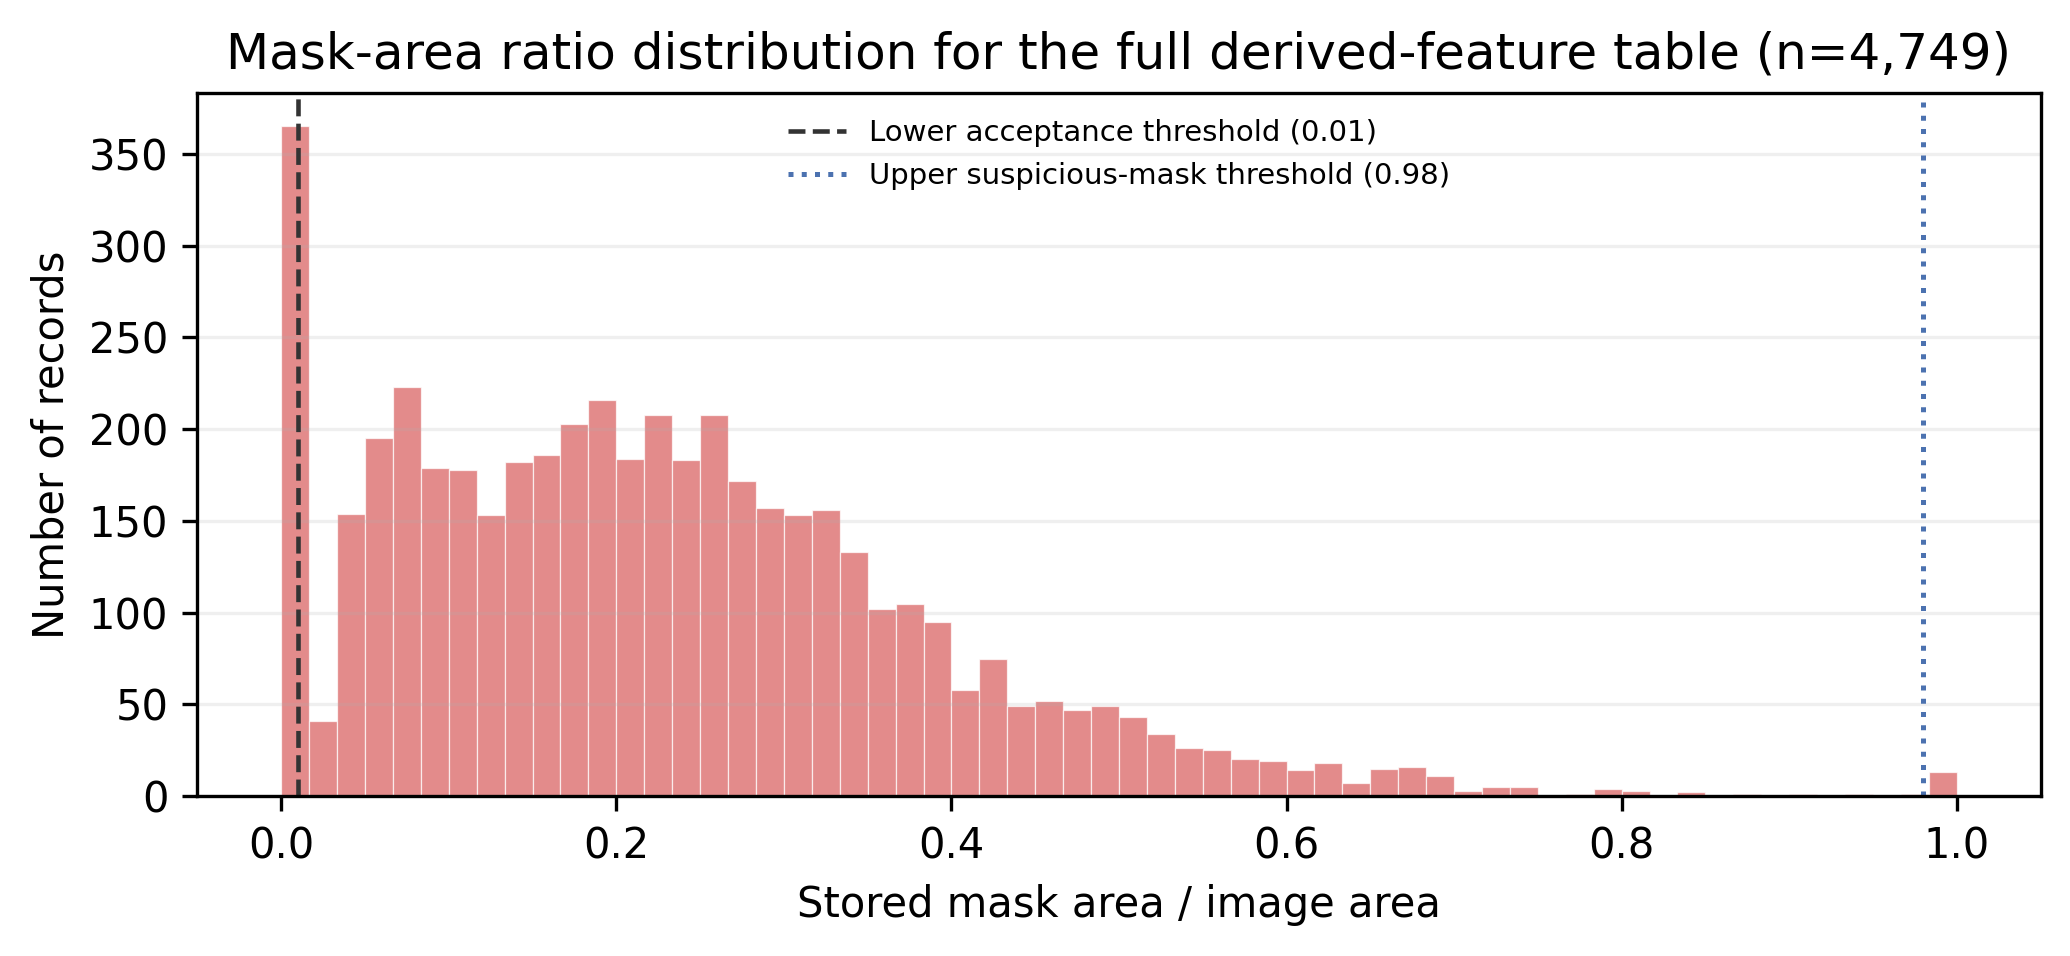
\includegraphics[width=\columnwidth]{figures/fig8_mask_ratio_distribution.png}
\caption{Distribution of stored mask-area ratios across the full derived table. The dashed line marks the 0.01 lower acceptance threshold. This plot visualizes the filter variable; it does not independently validate segmentation masks.}
\label{fig:maskdist}
\end{figure}

\subsection{Graph topology and representation size}

The five graph constructors produced different connectivity patterns: the spatial/regional graph was sparsest (19 edges), followed by the correlation graph (71--72 edges across folds), the kNN graph (81 edges), the feature-family graph (124 edges), and the hybrid graph (147 edges). Because all graphs share the same 38 nodes and the same initial labels, their height-zero representations were identical. The initial feature vocabulary had 114 dimensions, corresponding to three potential bins per feature.

WL refinement increased the number of distinct subtree-label dimensions, with the magnitude depending on graph topology and height. At each topology's macro-F1-selected height, average feature dimensions ranged from 12,938 for the correlation graph at height 2 to 129,065 for the hybrid graph at height 2. The feature-family graph at height 2 averaged 106,218 dimensions, whereas the spatial graph's selected height 3 averaged 15,077. At height 3, the hybrid representation averaged 259,337 dimensions. Figure~\ref{fig:topologies} shows that the hybrid and family topologies connect more feature pairs than the spatial design, while Table~\ref{tab:topology} summarises the construction rules and edge counts.

\subsection{Multiclass classification performance}

The best graph-kernel result by macro-F1 was obtained by the hybrid graph at WL height 2: accuracy 44.31\% $\pm$ 0.72\%, macro-F1 42.79\% $\pm$ 0.95\%, and weighted-F1 43.41\% $\pm$ 1.17\% (Table~\ref{tab:bestmodels}). The feature-family graph at height 2 and the kNN graph at height 2 were close, with macro-F1 values of 42.35\% $\pm$ 1.06\% and 42.33\% $\pm$ 1.15\%, respectively. The spatial/regional graph had the lowest best macro-F1 (39.30\% $\pm$ 1.01\%).

The flat Random Forest yielded the best overall performance among evaluated models, with accuracy 58.54\% $\pm$ 1.47\%, macro-F1 54.99\% $\pm$ 1.35\%, and weighted-F1 56.53\% $\pm$ 1.54\%. The linear SVM reached macro-F1 of 47.20\% $\pm$ 2.04\%, while the flat RBF SVM achieved 43.07\% $\pm$ 1.55\% and the $k$NN baseline achieved 41.02\% $\pm$ 1.05\%. Thus, no evaluated WL graph-kernel configuration improved on the flat Random Forest, linear SVM, or flat RBF SVM by macro-F1. The strongest graph-kernel model was 12.20 percentage points below the Random Forest in macro-F1 and 14.22 percentage points below it in accuracy. These differences are descriptive; we did not conduct a formal paired significance test.

\begin{table*}[!t]
\centering
\caption{Five-fold comparison of flat-feature baselines and the best WL height for each graph topology.}
\label{tab:bestmodels}
\scriptsize
\begin{tabular}{llrrr}
\toprule
Model / topology & Representation & Accuracy (\%) & Macro-F1 (\%) & Weighted-F1 (\%) \\
\midrule
Flat RBF SVM & Flat feature vector & 45.54 $\pm$ 1.97 & 43.07 $\pm$ 1.55 & 45.35 $\pm$ 2.19 \\
KNN (k=5) & Flat feature vector & 48.76 $\pm$ 0.85 & 41.02 $\pm$ 1.05 & 47.21 $\pm$ 0.97 \\
Linear SVM & Flat feature vector & 48.55 $\pm$ 2.10 & 47.20 $\pm$ 2.04 & 48.94 $\pm$ 2.08 \\
Random Forest & Flat feature vector & 58.54 $\pm$ 1.47 & 54.99 $\pm$ 1.35 & 56.53 $\pm$ 1.54 \\
Hybrid & WL height 2 & 44.31 $\pm$ 0.72 & 42.79 $\pm$ 0.95 & 43.41 $\pm$ 1.17 \\
Feature-family & WL height 2 & 43.86 $\pm$ 1.05 & 42.35 $\pm$ 1.06 & 43.09 $\pm$ 1.37 \\
Feature-similarity kNN & WL height 2 & 44.15 $\pm$ 1.07 & 42.33 $\pm$ 1.15 & 43.50 $\pm$ 1.36 \\
Correlation & WL height 2 & 41.08 $\pm$ 2.09 & 39.84 $\pm$ 2.89 & 40.77 $\pm$ 2.18 \\
Spatial/regional & WL height 3 & 40.30 $\pm$ 0.93 & 39.30 $\pm$ 1.01 & 39.94 $\pm$ 1.34 \\
\bottomrule
\end{tabular}
\smallskip
\begin{minipage}{0.97\linewidth}\footnotesize Entries are mean $\pm$ sample standard deviation across the same five folds. Graph heights were selected by mean macro-F1 within each topology from the pre-specified heights 0--3; the best-height values are therefore comparative rather than an independent external test.\end{minipage}
\end{table*}

\begin{figure*}[!t]
\centering
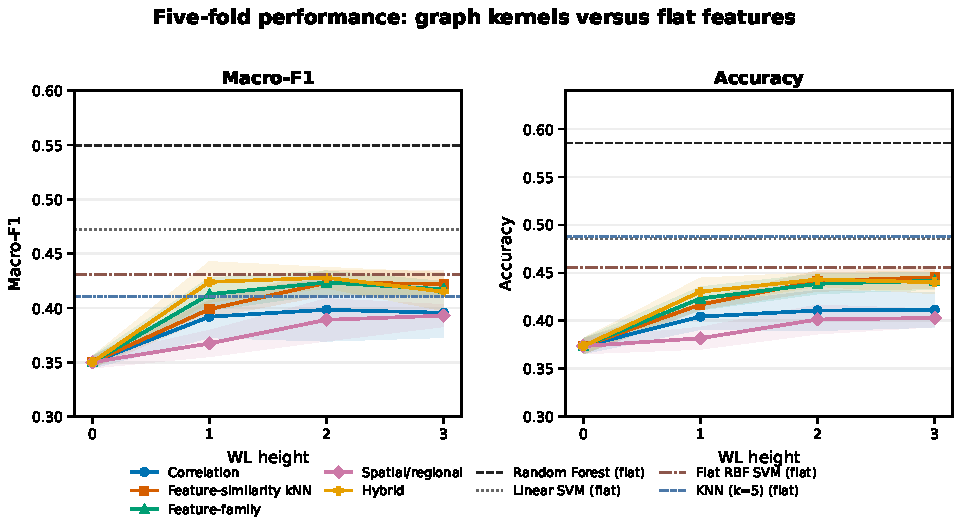
\includegraphics[width=0.97\textwidth]{figures/fig8_cv_performance.pdf}
\caption{Performance across WL heights, with horizontal lines for flat-feature baselines. Shaded regions indicate plus or minus one fold-level standard deviation.}
\label{fig:performance}
\end{figure*}

\subsection{Effect of WL height}

Performance depended on both topology and WL height (Table~\ref{tab:allheights}; Figure~\ref{fig:performance}). All topologies shared the same height-zero score (accuracy 37.36\% $\pm$ 0.80\%; macro-F1 35.01\% $\pm$ 0.54\%), as expected when topology is not yet incorporated through neighbourhood refinement. Raising the height to 1 improved macro-F1 for every topology. Macro-F1 peaked at height 2 for the correlation, kNN, feature-family, and hybrid topologies; the spatial/regional topology peaked at height 3. The hybrid graph produced the highest overall WL macro-F1 at height 2, whereas its macro-F1 decreased at height 3 (42.79\% to 41.50\%). For the family graph, macro-F1 likewise declined between heights 2 and 3 (42.35\% to 41.72\%).

Accuracy and macro-F1 did not always select the same representation. For example, the kNN graph's accuracy increased from 44.15\% at height 2 to 44.54\% at height 3, while its macro-F1 decreased slightly from 42.33\% to 42.23\%. This divergence is consistent with the importance of reporting class-balanced metrics in a multi-class dataset with uneven class counts. Overall, additional refinement increased representation dimensionality substantially, but did not produce a monotonic improvement in class-balanced prediction.

\begin{table*}[!t]
\centering
\caption{WL performance for all five topologies and four tested heights.}
\label{tab:allheights}
\scriptsize
\resizebox{\textwidth}{!}{%
\begin{tabular}{llrrrrr}
\toprule
Topology & Height & Mean edges & Accuracy (\%) & Macro-F1 (\%) & Weighted-F1 (\%) & Mean dimensions \\
\midrule
Correlation & 0 & 71.8 & 37.36 $\pm$ 0.80 & 35.01 $\pm$ 0.54 & 36.70 $\pm$ 1.16 & 114 \\
Correlation & 1 & 71.8 & 40.44 $\pm$ 1.34 & 39.20 $\pm$ 1.94 & 40.04 $\pm$ 1.70 & 3,641 \\
Correlation & 2 & 71.8 & 41.08 $\pm$ 2.09 & 39.84 $\pm$ 2.89 & 40.77 $\pm$ 2.18 & 12,938 \\
Correlation & 3 & 71.8 & 41.14 $\pm$ 1.82 & 39.56 $\pm$ 2.28 & 40.88 $\pm$ 1.93 & 32,144 \\
Feature-similarity kNN & 0 & 81.0 & 37.36 $\pm$ 0.80 & 35.01 $\pm$ 0.54 & 36.70 $\pm$ 1.16 & 114 \\
Feature-similarity kNN & 1 & 81.0 & 41.69 $\pm$ 0.51 & 39.90 $\pm$ 0.78 & 41.26 $\pm$ 0.88 & 5,295 \\
Feature-similarity kNN & 2 & 81.0 & 44.15 $\pm$ 1.07 & 42.33 $\pm$ 1.15 & 43.50 $\pm$ 1.36 & 51,276 \\
Feature-similarity kNN & 3 & 81.0 & 44.54 $\pm$ 1.16 & 42.23 $\pm$ 1.27 & 43.69 $\pm$ 1.35 & 133,259 \\
Feature-family & 0 & 124.0 & 37.36 $\pm$ 0.80 & 35.01 $\pm$ 0.54 & 36.70 $\pm$ 1.16 & 114 \\
Feature-family & 1 & 124.0 & 42.33 $\pm$ 1.21 & 41.27 $\pm$ 1.49 & 41.95 $\pm$ 1.72 & 22,012 \\
Feature-family & 2 & 124.0 & 43.86 $\pm$ 1.05 & 42.35 $\pm$ 1.06 & 43.09 $\pm$ 1.37 & 106,218 \\
Feature-family & 3 & 124.0 & 44.18 $\pm$ 0.89 & 41.72 $\pm$ 0.72 & 42.91 $\pm$ 1.24 & 236,490 \\
Spatial/regional & 0 & 19.0 & 37.36 $\pm$ 0.80 & 35.01 $\pm$ 0.54 & 36.70 $\pm$ 1.16 & 114 \\
Spatial/regional & 1 & 19.0 & 38.18 $\pm$ 1.14 & 36.74 $\pm$ 1.21 & 37.54 $\pm$ 1.43 & 1,118 \\
Spatial/regional & 2 & 19.0 & 40.14 $\pm$ 1.51 & 38.91 $\pm$ 1.95 & 39.59 $\pm$ 1.89 & 6,916 \\
Spatial/regional & 3 & 19.0 & 40.30 $\pm$ 0.93 & 39.30 $\pm$ 1.01 & 39.94 $\pm$ 1.34 & 15,077 \\
Hybrid & 0 & 147.0 & 37.36 $\pm$ 0.80 & 35.01 $\pm$ 0.54 & 36.70 $\pm$ 1.16 & 114 \\
Hybrid & 1 & 147.0 & 43.04 $\pm$ 1.42 & 42.40 $\pm$ 1.87 & 42.56 $\pm$ 1.96 & 26,432 \\
Hybrid & 2 & 147.0 & 44.31 $\pm$ 0.72 & 42.79 $\pm$ 0.95 & 43.41 $\pm$ 1.17 & 129,065 \\
Hybrid & 3 & 147.0 & 44.02 $\pm$ 1.19 & 41.50 $\pm$ 1.75 & 42.48 $\pm$ 1.56 & 259,337 \\
\bottomrule
\end{tabular}%
}
\smallskip
\begin{minipage}{0.96\linewidth}\footnotesize Mean dimensions are the average number of training-vocabulary WL count features across folds. Scores are percentages and entries are mean $\pm$ sample standard deviation. Height zero uses the same initial node labels for each topology.\end{minipage}
\end{table*}

\section{Discussion}

\subsection{Main finding: topology matters, but did not beat the flat baselines}

This comparison shows that graph construction is not a neutral implementation detail. At a fixed node inventory, the choice of edges changes WL neighbourhood signatures, the number of distinct subtree patterns, and the resulting kernel. The hybrid graph at height 2 had the strongest graph-kernel macro-F1, but all tested graph-kernel configurations remained below the flat Random Forest and the two flat SVM baselines by macro-F1. The evidence therefore does not support the claim that representing these 38 descriptors as graphs automatically improves the full 57-class task.

One interpretation is that the handcrafted features already provide a useful nonlinear or ensemble-friendly representation of the target categories. The Random Forest can model feature interactions through tree partitions without requiring an explicit graph topology, while a WL kernel converts each leaf's descriptor profile into counts of discrete local structures. Quantile binning discards within-bin magnitude differences, and the graph representation may amplify topology-specific patterns that are not consistently aligned with crop--condition class boundaries. These are plausible explanations, not mechanisms directly proven by the current experiments.

The relatively close performance of the hybrid, family, and kNN graph variants also suggests that no single edge design was decisively superior. The hybrid graph contains more edges and produced a large WL vocabulary, yet it improved macro-F1 over the family and kNN variants by less than one percentage point at their best heights. Without repeated outer resampling or paired statistical tests, this small difference should not be interpreted as evidence of a robust winner. The result is better viewed as a practical benchmark: for the included feature table and fixed classifier settings, a flat Random Forest is the more effective default.

\subsection{Why kernel height and metric choice matter}

The shared height-zero result confirms that every topology begins from the same node labels; topology only contributes after neighbour labels are incorporated. The improvement from height 0 to heights 1--2 indicates that local relationships between feature bins provide additional discriminatory information for some classes. The decline at higher height for several topologies is compatible with increasingly specific label configurations, which can become rare in validation folds and increase sparsity. This behaviour supports treating WL height as a model-design choice rather than assuming that deeper refinement is always better.

Accuracy weights every sample equally, whereas macro-F1 weights classes equally after computing their F1 values. In an imbalanced 57-class problem, a model can raise accuracy by improving predictions for common classes while losing recall or precision on rarer categories. For that reason, macro-F1 was used to identify the best height within each graph topology, while all metrics are reported to make the trade-offs visible. The selected height was chosen from the four pre-specified values; however, the reported CV scores should still be interpreted as model-comparison estimates, not final external generalization estimates.

\subsection{Segmentation quality is a modelling concern, not only an image-processing detail}

The retention audit is an important result in its own right. A 7.62\% overall exclusion rate could appear modest if considered alone, but crop-level acceptance ranged from 72.68\% to 99.90\%, and the LM condition retained only about half its records. If the probability of passing a mask-quality threshold depends on crop or stress morphology, excluding poor masks can change the class distribution before any model is trained. It can also remove difficult but potentially important examples and make downstream estimates optimistic for the original data population. The current study cannot quantify that performance shift because rejected images were not included in the model-level comparison.

Future work should use a segmentation system that is evaluated across stress categories, audit failed masks by expert inspection, and either recover or explicitly model the rejected records. Sensitivity analysis over mask thresholds can help diagnose retention effects, but threshold changes alone do not guarantee correct leaf segmentation. In particular, tomato and LM samples should be reviewed because the stored audit identifies them as low-retention groups. Reporting only model accuracy after filtering would overlook this limitation.

\subsection{Relation to prior work}

Previous plant phenotyping research has explored feature-based classification, deep neural networks, and high-throughput imaging pipelines \cite{Mohanty2016,Gill2022,Pacal2024}. The release of OLID-I broadened benchmark coverage beyond a small number of disease-only categories by including multiple crops and combined stress labels \cite{Orka2023}. Recent studies have investigated graph kernels for image-derived traits and hybrid neural architectures on OLID-I \cite{Sriram2026,Karthikeyan2026}. The current work is complementary: it isolates one design question---how alternative feature-graph topologies and WL heights behave when the same handcrafted descriptors and train/validation partitions are held fixed. Since differences in datasets, labels, split protocol, feature pipelines, and model tuning prevent direct comparisons with the published scores in those studies, we do not claim superiority or inferiority relative to their reported metrics.

\subsection{Limitations and recommended next steps}

Several limitations constrain the conclusions. The leaf-image montage is illustrative only and is not the basis for any reported score; metrics are computed from the full derived-feature table rather than from the pictured examples alone. First, experiments use a stored derived-feature table rather than a fresh extraction from every raw image; independent end-to-end reproduction requires the original images and a clean rerun of the segmentation and feature-extraction notebooks. Second, only accepted masks enter classification. The results therefore do not evaluate rejected samples or deployment robustness under imperfect segmentation. Third, the study uses one stratified five-fold partition, fixed hyperparameters, and no independent external dataset. Standard deviations across folds are not confidence intervals, and the current results do not establish statistical significance. Fourth, handcrafted descriptors are not equivalent to learned visual representations, and some descriptors have implementation-specific limitations: notably, GLCM values are computed on a bounding-box crop, and derived yellow/green ratios should be interpreted as pipeline-specific proxies rather than calibrated pigment measurements. Fifth, the graph-kernel vocabulary grows rapidly at larger heights, particularly for the family and hybrid graphs, increasing memory and computation while offering no reliable macro-F1 gain. Finally, source notebooks contained cached WL metrics that did not match the patched feature-identity logic; this paper reports a clean re-analysis and includes its fold-level outputs and scripts to make the reported values traceable. Because topology-specific heights are selected using these same folds, nested or repeated cross-validation is needed to estimate the performance of a fully selected graph model without selection optimism.

A rigorous follow-up should (i) rerun the full extraction from public raw images; (ii) retain and manually audit segmentation failures; (iii) evaluate multiple seeds or repeated nested cross-validation for model selection; (iv) compare against tuned tree ensembles and image-based deep models using identical splits; (v) report class-wise precision/recall and confusion matrices; (vi) investigate alternative descriptors and continuous or hybrid graph-node representations; and (vii) evaluate an external field dataset before drawing conclusions about agronomic use.

\subsection{Conclusions}

For the supplied OLID-I-derived feature table, graph topology and WL height changed performance, with the hybrid graph at height 2 providing the strongest graph-kernel result (macro-F1 42.79\%). However, the flat Random Forest achieved higher accuracy and macro-F1, so these experiments do not demonstrate a predictive advantage from the evaluated graph kernels. The accompanying selection audit found markedly different acceptance rates across crops and conditions, identifying a data-quality issue that should be addressed before using filtered-image results as evidence of general plant-stress recognition. The primary contribution is a reproducible comparison with explicit limits, which provides a sound basis for a more carefully validated graph-based phenotyping study.

\section*{Data and Code Availability}
The original OLID-I dataset is described by Orka et al.~\cite{Orka2023} and is available through the dataset record at \url{https://doi.org/10.5281/zenodo.8105154}. The derived feature table, fold assignments, fold-level results, feature dictionary, and analysis scripts used for this draft are included in the review package supplied to the team. A public repository URL/DOI has not yet been assigned and must be added before submission. Raw images were not bundled in the supplied project ZIP and must be obtained from the original dataset release for full image-to-feature reproduction.

\section*{Ethics Statement}
This study analyses an existing public collection of plant-leaf images and their derived numerical descriptors. No human participants or vertebrate animals were involved. The authors should confirm any dataset-specific licensing or permissions required for redistribution of derived records and images.

% \section*{Author Contributions}
% \textbf{[AUTHOR TEAM: complete this section before submission using the journal's required contribution taxonomy. Do not infer authorship or contributions from notebook names alone.]}

% \section*{Funding}
% \textbf{[AUTHOR TEAM: insert the accurate funder name and grant number, or state that no external funding was received if that is correct.]}

% \section*{Competing Interests}
% \textbf{[AUTHOR TEAM: confirm whether any competing interests exist and replace this instruction with the journal's required statement.]}

\section*{Acknowledgments}
The authors acknowledge the OLID-I dataset creators for making a diverse plant-stress image benchmark publicly available~\cite{Orka2023}. Additional institutional or technical acknowledgments should be added by the team if applicable.

% \section*{Generative-AI Disclosure}
% OpenAI ChatGPT (model GPT-6; OpenAI; accessed 19 October 2026) assisted with manuscript organization, text drafting, and the preparation of scripts for aggregating the supplied fold-level model results and creating figures. Numerical results reported in the manuscript were computed from the supplied feature table and saved source files using the scripts included with this draft; all calculations and references should be independently checked by the author team before submission.

\section*{Supplementary material}
The supplementary folder contains the 38-feature dictionary, feature-family counts, a class-level mask-acceptance audit, and machine-readable fold-level performance outputs. The analysis folder contains fold assignments, full fold-level baseline and WL results, summary tables, and run metadata. The README documents how to reproduce the aggregation and figures.

% \balance
\begin{thebibliography}{00}
\bibitem{Mohanty2016} S. P. Mohanty, D. P. Hughes, and M. Salath\'e, ``Using deep learning for image-based plant disease detection,'' \emph{Frontiers in Plant Science}, vol. 7, Art. no. 1419, 2016, doi: 10.3389/fpls.2016.01419.
\bibitem{Gill2022} T. Gill, S. K. Gill, D. K. Saini, Y. Chopra, J. P. de Koff, and K. S. Sandhu, ``A comprehensive review of high throughput phenotyping and machine learning for plant stress phenotyping,'' \emph{Phenomics}, vol. 2, pp. 156--183, 2022, doi: 10.1007/s43657-022-00048-z.
\bibitem{Pacal2024} I. Pacal \emph{et al.}, ``A systematic review of deep learning techniques for plant diseases,'' \emph{Artificial Intelligence Review}, vol. 57, Art. no. 304, 2024, doi: 10.1007/s10462-024-10944-7.
\bibitem{Orka2023} N. A. Orka, M. N. Uddin, F. M. Toushique, and M. S. Hossain, ``OLID I: An open leaf image dataset for plant stress recognition,'' \emph{Frontiers in Plant Science}, vol. 14, Art. no. 1251888, 2023, doi: 10.3389/fpls.2023.1251888.
\bibitem{Karthikeyan2026} A. Karthikeyan and S. Sundar, ``Q-TriLSTM-Vision: A quantum-interference-augmented tri-stream LSTM for multi-label plant stress recognition on the OLID-I benchmark,'' \emph{Frontiers in Plant Science}, vol. 17, Art. no. 1903924, 2026, doi: 10.3389/fpls.2026.1903924.
\bibitem{Sriram2026} S. Sriram and T. Ramraj, ``Perceptual graph kernels for image-derived plant trait interaction analysis in precision agriculture,'' \emph{Frontiers in Plant Science}, vol. 17, Art. no. 1822052, 2026, doi: 10.3389/fpls.2026.1822052.
\bibitem{Shervashidze2011} N. Shervashidze, P. Schweitzer, E. J. van Leeuwen, K. Mehlhorn, and K. M. Borgwardt, ``Weisfeiler--Lehman graph kernels,'' \emph{Journal of Machine Learning Research}, vol. 12, pp. 2539--2561, 2011.
\bibitem{Otsu1979} N. Otsu, ``A threshold selection method from gray-level histograms,'' \emph{IEEE Transactions on Systems, Man, and Cybernetics}, vol. 9, no. 1, pp. 62--66, 1979, doi: 10.1109/TSMC.1979.4310076.
\bibitem{Haralick1973} R. M. Haralick, K. Shanmugam, and I. Dinstein, ``Textural features for image classification,'' \emph{IEEE Transactions on Systems, Man, and Cybernetics}, vol. SMC-3, no. 6, pp. 610--621, 1973, doi: 10.1109/TSMC.1973.4309314.
\bibitem{Cortes1995} C. Cortes and V. Vapnik, ``Support-vector networks,'' \emph{Machine Learning}, vol. 20, no. 3, pp. 273--297, 1995, doi: 10.1007/BF00994018.
\bibitem{Breiman2001} L. Breiman, ``Random forests,'' \emph{Machine Learning}, vol. 45, no. 1, pp. 5--32, 2001, doi: 10.1023/A:1010933404324.
\bibitem{Pedregosa2011} F. Pedregosa \emph{et al.}, ``Scikit-learn: Machine learning in Python,'' \emph{Journal of Machine Learning Research}, vol. 12, pp. 2825--2830, 2011.
\end{thebibliography}
\end{document}
